\section{Razvoj programskog jezika Clojure}
\label{sec:razvoj}

Clojure je razvijen od strane Riča Hikija(engl. \textit{Rich Hickey})\cite{clojure}, tvorca .Lisp-a i drugih Lisp-olikih jezika, pokušaja povezivanja sa Javom. Prva verzija je zvanično objavljena 16.10.2007. iako je jezik postojao već dve godine. U tabeli \ref{tab:verzije}, hronološki su predstavljene sve objavljene verzije i njihove glavne odlike.


\begin{table}[h!]
\begin{center}
\begin{tabular}{|c|c|c|} \hline
\textbf{Verzija} & \textbf{Datum izlaska} & \textbf{Novine}\\ \hline
 & 16.10.2007. & Prvo zvanično objavljivanje \\ \hline
1.0 & 04.05.2009. & Prva stabilna verzija\\ \hline
1.1 & 31.12.2009. & Operator \texttt{future} za sinhronizaciju\\ \hline
1.2 & 19.08.2010. & Protokoli\\ \hline
1.3 & 23.09.2011. & Napredna podrška za primitive\\ \hline
1.4 & 15.04.2012. & Literali čitača\\ \hline
1.5 & 01.03.2013. & Reduktori\\ \hline
1.6 & 25.03.2014. & Java API, unapređeni heš algoritmi\\ \hline
1.7 & 30.06.2015. & Uslovi za čitač, transduktori\\ \hline
1.8 & 19.01.2016. & Funkcije za niske, direktno linkovanje\\ \hline
1.9 & 08.12.2017. & Alati komandne linije\\ \hline
\textbf{1.10} & 17.12.2018. & Izveštaji o greškama, Java kompatibilnost\\ \hline
\end{tabular}
\caption{Objavljene verzije\cite{clojure_release_1}\cite{clojure_release_2}}
\label{tab:verzije}
\end{center}
\end{table}

Razvoju jezika umnogome je doprinela njegova zajednica, koja je aktivna od trenutka kada se on pojavio. Clojure konferencije, od kojih su najposećenije one u Sjedinjenim državama i evropske konferencije, organizuju se svake godine širom planete.

\subsection{Odnos sa drugim programskim jezicima}
\label{subsec:drugijezici}

Kao odgovor na pitanje zašto je osmislio još jedan Lisp-oliki jezik, njegov tvorac je odgovorio: "U osnovi, bio mi je potreban Lisp za funkcionalno programiranje, simbiotičan sa osnovnom Java platformom i dizajniran za konkurentnost. Nisam mogao da pronađem takav jezik, pa sam ga stvorio"\cite{clojure}.


 \begin{figure}[h]
     % 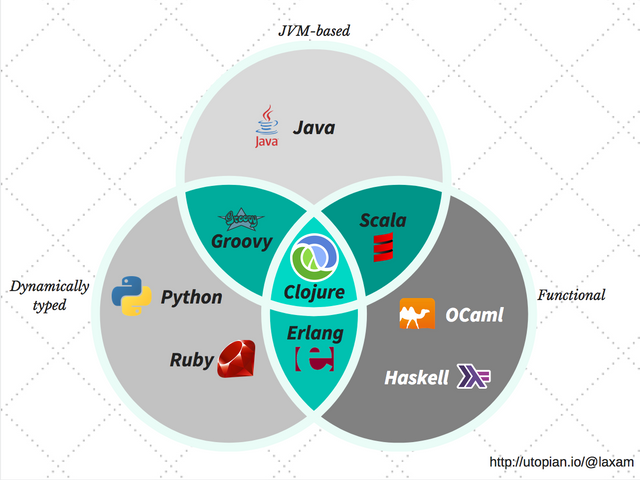
\includegraphics[width=0.6\textwidth]{Slike/clojure.png}
     \centering
     % \hspace{2.5cm}
     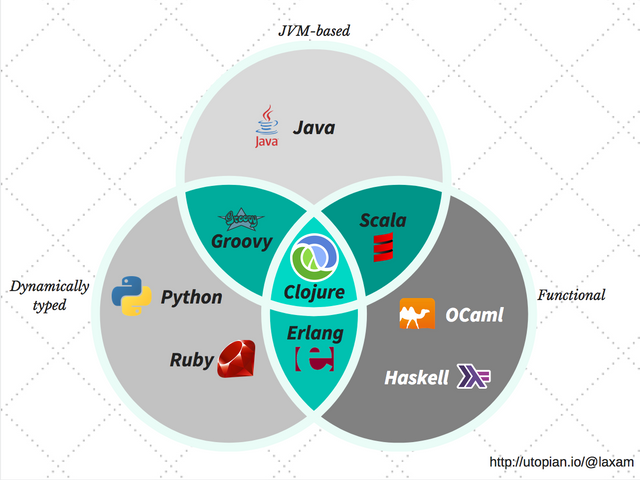
\includegraphics[width=0.5\textwidth]{Slike/clojure.png}
     \caption{Odnos Clojure-a i drugih programskih jezika}
     \label{fig:clojure_ostali}
 \end{figure}

Kao direktan Lisp-ov potomak, smestio se u stablu \ref{fig:stablo} programskih jezika  kao "mlađi brat" funkcionalnih jezika kao što su Smalltalk i Dylan.

\begin{figure}[ht]
    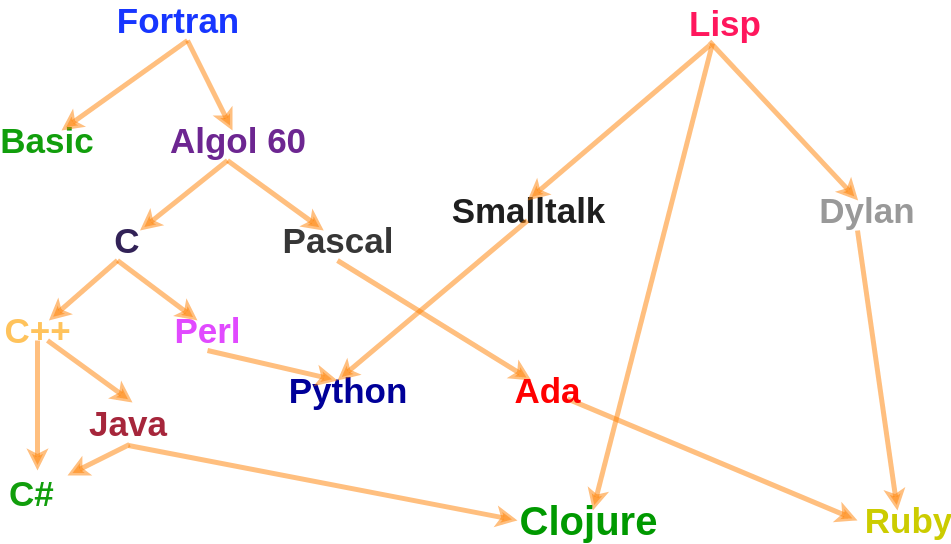
\includegraphics[width=0.6\textwidth]{Slike/stablo.png}
    \centering
    \caption{Clojure u stablu programskih jezika}
    \label{fig:stablo}
\end{figure}